\documentclass[a4paper,12pt]{article}
\usepackage{graphicx}
\usepackage{hyperref}
\usepackage{caption}
\usepackage{listings}
\begin{document}

\title{The exponential function}
\author{Maria Hinge Pedersen}
\date{\today}
\maketitle
\section{Introduction of the exponential function}
The exponential function is a mathematical function denoted by $f(x)=\exp(x)$ or $e^x$ (where the argument $x$ is written as an exponentiation).
It is an important function in both mathematics and physics.
It is defined in severals different ways, but for this introduction the following definition is used:
\begin{equation} \label{eq:def}
	exp(x) = \sum_{k=0}^{\infty} \frac{x^k}{k!}= 1+x+\frac{x^2}{x}+\frac{x^3}{6}+\frac{x^4}{24}+\ldots
\end{equation}
Its value at $1$, $e = \exp(1)$ is a mathematical constant known as Euler's number. \footnote{https://en.wikipedia.org/wiki/Exponential\_function} \

To implement the function, the code shown in figure \ref{code:exp} is used.

\begin{figure}\label{fig:plot}
	\centering
		% GNUPLOT: LaTeX picture with Postscript
\begingroup
  \makeatletter
  \providecommand\color[2][]{%
    \GenericError{(gnuplot) \space\space\space\@spaces}{%
      Package color not loaded in conjunction with
      terminal option `colourtext'%
    }{See the gnuplot documentation for explanation.%
    }{Either use 'blacktext' in gnuplot or load the package
      color.sty in LaTeX.}%
    \renewcommand\color[2][]{}%
  }%
  \providecommand\includegraphics[2][]{%
    \GenericError{(gnuplot) \space\space\space\@spaces}{%
      Package graphicx or graphics not loaded%
    }{See the gnuplot documentation for explanation.%
    }{The gnuplot epslatex terminal needs graphicx.sty or graphics.sty.}%
    \renewcommand\includegraphics[2][]{}%
  }%
  \providecommand\rotatebox[2]{#2}%
  \@ifundefined{ifGPcolor}{%
    \newif\ifGPcolor
    \GPcolorfalse
  }{}%
  \@ifundefined{ifGPblacktext}{%
    \newif\ifGPblacktext
    \GPblacktexttrue
  }{}%
  % define a \g@addto@macro without @ in the name:
  \let\gplgaddtomacro\g@addto@macro
  % define empty templates for all commands taking text:
  \gdef\gplbacktext{}%
  \gdef\gplfronttext{}%
  \makeatother
  \ifGPblacktext
    % no textcolor at all
    \def\colorrgb#1{}%
    \def\colorgray#1{}%
  \else
    % gray or color?
    \ifGPcolor
      \def\colorrgb#1{\color[rgb]{#1}}%
      \def\colorgray#1{\color[gray]{#1}}%
      \expandafter\def\csname LTw\endcsname{\color{white}}%
      \expandafter\def\csname LTb\endcsname{\color{black}}%
      \expandafter\def\csname LTa\endcsname{\color{black}}%
      \expandafter\def\csname LT0\endcsname{\color[rgb]{1,0,0}}%
      \expandafter\def\csname LT1\endcsname{\color[rgb]{0,1,0}}%
      \expandafter\def\csname LT2\endcsname{\color[rgb]{0,0,1}}%
      \expandafter\def\csname LT3\endcsname{\color[rgb]{1,0,1}}%
      \expandafter\def\csname LT4\endcsname{\color[rgb]{0,1,1}}%
      \expandafter\def\csname LT5\endcsname{\color[rgb]{1,1,0}}%
      \expandafter\def\csname LT6\endcsname{\color[rgb]{0,0,0}}%
      \expandafter\def\csname LT7\endcsname{\color[rgb]{1,0.3,0}}%
      \expandafter\def\csname LT8\endcsname{\color[rgb]{0.5,0.5,0.5}}%
    \else
      % gray
      \def\colorrgb#1{\color{black}}%
      \def\colorgray#1{\color[gray]{#1}}%
      \expandafter\def\csname LTw\endcsname{\color{white}}%
      \expandafter\def\csname LTb\endcsname{\color{black}}%
      \expandafter\def\csname LTa\endcsname{\color{black}}%
      \expandafter\def\csname LT0\endcsname{\color{black}}%
      \expandafter\def\csname LT1\endcsname{\color{black}}%
      \expandafter\def\csname LT2\endcsname{\color{black}}%
      \expandafter\def\csname LT3\endcsname{\color{black}}%
      \expandafter\def\csname LT4\endcsname{\color{black}}%
      \expandafter\def\csname LT5\endcsname{\color{black}}%
      \expandafter\def\csname LT6\endcsname{\color{black}}%
      \expandafter\def\csname LT7\endcsname{\color{black}}%
      \expandafter\def\csname LT8\endcsname{\color{black}}%
    \fi
  \fi
    \setlength{\unitlength}{0.0500bp}%
    \ifx\gptboxheight\undefined%
      \newlength{\gptboxheight}%
      \newlength{\gptboxwidth}%
      \newsavebox{\gptboxtext}%
    \fi%
    \setlength{\fboxrule}{0.5pt}%
    \setlength{\fboxsep}{1pt}%
    %\definecolor{tbcol}{rgb}{1,1,1}%
\begin{picture}(4320.00,3024.00)%
    \gplgaddtomacro\gplbacktext{%
      \csname LTb\endcsname%%
      \put(814,767){\makebox(0,0)[r]{\strut{}$0$}}%
      \put(814,1022){\makebox(0,0)[r]{\strut{}$20$}}%
      \put(814,1276){\makebox(0,0)[r]{\strut{}$40$}}%
      \put(814,1531){\makebox(0,0)[r]{\strut{}$60$}}%
      \put(814,1785){\makebox(0,0)[r]{\strut{}$80$}}%
      \put(814,2040){\makebox(0,0)[r]{\strut{}$100$}}%
      \put(814,2294){\makebox(0,0)[r]{\strut{}$120$}}%
      \put(814,2549){\makebox(0,0)[r]{\strut{}$140$}}%
      \put(814,2803){\makebox(0,0)[r]{\strut{}$160$}}%
      \put(1009,484){\makebox(0,0){\strut{}$-6$}}%
      \put(1484,484){\makebox(0,0){\strut{}$-4$}}%
      \put(1959,484){\makebox(0,0){\strut{}$-2$}}%
      \put(2435,484){\makebox(0,0){\strut{}$0$}}%
      \put(2910,484){\makebox(0,0){\strut{}$2$}}%
      \put(3385,484){\makebox(0,0){\strut{}$4$}}%
      \put(3860,484){\makebox(0,0){\strut{}$6$}}%
    }%
    \gplgaddtomacro\gplfronttext{%
      \csname LTb\endcsname%%
      \put(209,1785){\rotatebox{-270}{\makebox(0,0){\strut{}$t$}}}%
      \put(2434,154){\makebox(0,0){\strut{}$x$}}%
      \put(2873,2630){\makebox(0,0)[r]{\strut{}$e^x$}}%
      \put(2873,2410){\makebox(0,0)[r]{\strut{}Tabulated data}}%
    }%
    \gplbacktext
    \put(0,0){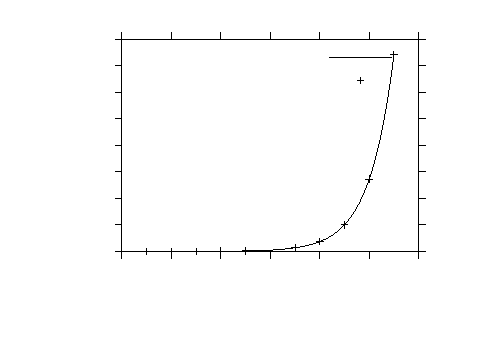
\includegraphics[width={216.00bp},height={151.20bp}]{exp_plot}}%
    \gplfronttext
  \end{picture}%
\endgroup

	\caption{Plot of the exponential function by the code.}
\end{figure}

If the argument is below $0$, the function returns $1/e^x$ which is equivalent to $e^{-x}$.
For relatively large $x$ (i.e. $x>$ 1/8) the recursive definition $\exp{x}=(\exp{x/2})^2$ is used, while the Taylor expansion in equation \ref{eq:def} can be used for smaller, but positive values of $x$.

The implementation is then tested by plotting it against known table values, which is done in figure \ref{code:exp}.
And it works.

\begin{lstlisting}[breaklines]
static double ex(double x){
if(x<0)return 1/ex(-x);
if(x>1.0/8)return Pow(ex(x/2),2);
return 1+x*(1+x/2*(1+x/3*(1+x/4*(1+x/5*(1+x/6*(1+x/7*(1+x/8*(1+x/9*(1+x/10)))))))));
}
\end{lstlisting} \label{code:exp}

\end{document}
